\documentclass{beamer}
\usepackage[outputdir=build]{minted}
\usepackage[skins,minted,breakable]{tcolorbox}
\usepackage[spanish]{babel}
\usepackage{subcaption}
\usetikzlibrary{chains}
\usetikzlibrary{matrix,backgrounds}
\usepackage{multirow}
\usepackage{multicol}
\usepackage{subcaption}
\usepackage{xcolor}
\usepackage{pgfgantt}

\usepackage{forest}
\usepackage{color, colortbl}
\usepackage{pgfgantt}
\graphicspath{ {../img/} {../../LaTeX/img/} {/home/csp98/latex/img/}}
\selectlanguage{spanish}
\usepackage[utf8]{inputenc}
\usetheme{PaloAlto}
\setbeamerfont{section in sidebar}{size=\fontsize{2}{4}\selectfont}
\setbeamerfont{subsection in sidebar}{size=\fontsize{2}{3}\selectfont}
\setbeamerfont{subsubsection in sidebar}{size=\fontsize{2}{2}\selectfont}

\setbeamerfont{section in toc}{size=\footnotesize}
\setbeamerfont{subsection in toc}{size=\scriptsize}
\setbeamerfont{subsubsection in toc}{size=\tiny}


\title{Práctica 3}
\date{6 de abril de 2018}
\subtitle{Formas de sumar \textit{n}}

\author{María Jesús López Salmerón \\ Nazaret Román Guerrero \\ Laura Hernández Muñoz \\ José Baena Cobos  \\ Carlos Sánchez Páez}

\makeatletter
  \setbeamertemplate{sidebar \beamer@sidebarside}%{sidebar theme}
  {
    \beamer@tempdim=\beamer@sidebarwidth%
    \advance\beamer@tempdim by -6pt%
    \insertverticalnavigation{\beamer@sidebarwidth}%
    \vfill
    \ifx\beamer@sidebarside\beamer@lefttext%
    \else%
      \usebeamercolor{normal text}%
      \llap{\usebeamertemplate***{navigation symbols}\hskip0.1cm}%
      \vskip2pt%
    \fi%
}%
\makeatother

\subject{Algorítmica}
\AtBeginSection[]
  {
     \begin{frame}<beamer>
     \frametitle{Índice}
     \tableofcontents[currentsection]
     \end{frame}
  }
\AtBeginSubsection[]
{
  \begin{frame}<beamer>{Índice}
    \tableofcontents[currentsection,currentsubsection]
  \end{frame}
}

\AtBeginSubsubsection[]
{
  \begin{frame}<beamer>{Índice}
    \tableofcontents[currentsection,currentsubsection]
  \end{frame}
}

% Let's get started
\begin{document}
\centering
\begin{frame}
  \titlepage
\end{frame}

\begin{frame}{Índice}
  \tableofcontents
  % You might wish to add the option [pausesections]
\end{frame}

\section{Presentación del problema}


\begin{frame}[fragile]{Formas de sumar $n$}
Dado un $n \in \mathbb{N}$, hallar todas las posibles formas en las que la suma de los elementos de un conjunto ordenado de forma ascendente sea $n$.
\end{frame}

\begin{frame}[fragile]{Ejemplo ($n=8$)}
\begin{itemize}
	\item 1 + 7
\end{itemize}
\end{frame}

\begin{frame}[fragile]{Ejemplo ($n=8$)}
\begin{itemize}
	\item 1 + 7
	\item 2 + 6
\end{itemize}
\end{frame}

\begin{frame}[fragile]{Ejemplo ($n=8$)}
\begin{itemize}
	\item 1 + 7
	\item 2 + 6
	\item 3 + 5
\end{itemize}
\end{frame}

\begin{frame}[fragile]{Ejemplo ($n=8$)}
\begin{itemize}
	\item 1 + 7
	\item 2 + 6
	\item 3 + 5
	\item 1 + 2 + 5
\end{itemize}
\end{frame}

\begin{frame}[fragile]{Ejemplo ($n=8$)}
\begin{itemize}
	\item 1 + 7
	\item 2 + 6
	\item 3 + 5
	\item 1 + 2 + 5
	\item 1 + 3 + 4
\end{itemize}
\end{frame}

\begin{frame}[fragile]{Ejemplo ($n=8$)}
\begin{itemize}
	\item 1 + 7
	\item 2 + 6
	\item 3 + 5
	\item 1 + 2 + 5
	\item 1 + 3 + 4
	\item 8	
\end{itemize}
\end{frame}

\section{Algoritmos implementados}

\subsection{Fuerza bruta}
\begin{frame}[fragile]{Fuerza bruta ($n=3$)}
\begin{figure}[H]

\begin{tikzpicture}[font=\ttfamily,
array/.style={matrix of nodes,nodes={draw, minimum size=7mm, fill=blue!30},column sep=-\pgflinewidth, row sep=0.5mm, nodes in empty cells,
row 1/.style={nodes={draw=none, fill=none, minimum size=5mm}}}]

\matrix[array] (array) {
0 & 1 & 2 \\
  &   &     \\};
\node at (array-2-1) {1};
\node at (array-2-2) {2};
\node at (array-2-3) {3};

\draw[<->]([yshift=-3mm]array-2-1.south west) -- node[below] {Conjunto} ([yshift=-3mm]array-2-3.south east);
\end{tikzpicture}

\begin{tikzpicture}[font=\ttfamily,
array/.style={matrix of nodes,nodes={draw, minimum size=7mm, fill=blue!30},column sep=-\pgflinewidth, row sep=0.5mm, nodes in empty cells,
row 1/.style={nodes={draw=none, fill=none, minimum size=5mm}}}]

\matrix[array] (array) {
0 & 1 & 2 \\
  &   &     \\};
\node at (array-2-1) {?};
\node at (array-2-2) {?};
\node at (array-2-3) {?};

\draw[<->]([yshift=-3mm]array-2-1.south west) -- node[below] {Tuplas} ([yshift=-3mm]array-2-3.south east);
\end{tikzpicture}
\end{figure}
Estado inicial
\end{frame}

\begin{frame}[fragile]{Fuerza bruta ($n=3$)}
\begin{figure}[H]

\begin{tikzpicture}[font=\ttfamily,
array/.style={matrix of nodes,nodes={draw, minimum size=7mm, fill=blue!30},column sep=-\pgflinewidth, row sep=0.5mm, nodes in empty cells,
row 1/.style={nodes={draw=none, fill=none, minimum size=5mm}}}]

\matrix[array] (array) {
0 & 1 & 2 \\
  &   &     \\};
\node at (array-2-1) {1};
\node at (array-2-2) {2};
\node at (array-2-3) {3};

\draw[<->]([yshift=-3mm]array-2-1.south west) -- node[below] {Conjunto} ([yshift=-3mm]array-2-3.south east);
\end{tikzpicture}

\begin{tikzpicture}[font=\ttfamily,
array/.style={matrix of nodes,nodes={draw, minimum size=7mm, fill=blue!30},column sep=-\pgflinewidth, row sep=0.5mm, nodes in empty cells,
row 1/.style={nodes={draw=none, fill=none, minimum size=5mm}}}]

\matrix[array] (array) {
0 & 1 & 2 \\
  &   &     \\};
\node at (array-2-1) {2};
\node at (array-2-2) {?};
\node at (array-2-3) {?};

\draw[<->]([yshift=-3mm]array-2-1.south west) -- node[below] {Tuplas} ([yshift=-3mm]array-2-3.south east);
\end{tikzpicture}
\end{figure}
Inicializamos tuplas[0]
\end{frame}

\begin{frame}[fragile]{Fuerza bruta ($n=3$)}
\begin{figure}[H]
\begin{tikzpicture}[font=\ttfamily,
array/.style={matrix of nodes,nodes={draw, minimum size=7mm, fill=blue!30},column sep=-\pgflinewidth, row sep=0.5mm, nodes in empty cells,
row 1/.style={nodes={draw=none, fill=none, minimum size=5mm}}}]

\matrix[array] (array) {
0 & 1 & 2 \\
  &   &     \\};
\node at (array-2-1) {1};
\node at (array-2-2) {2};
\node at (array-2-3) {3};

\draw[<->]([yshift=-3mm]array-2-1.south west) -- node[below] {Conjunto} ([yshift=-3mm]array-2-3.south east);
\end{tikzpicture}

\begin{tikzpicture}[font=\ttfamily,
array/.style={matrix of nodes,nodes={draw, minimum size=7mm, fill=blue!30},column sep=-\pgflinewidth, row sep=0.5mm, nodes in empty cells,
row 1/.style={nodes={draw=none, fill=none, minimum size=5mm}}}]

\matrix[array] (array) {
0 & 1 & 2 \\
  &   &     \\};
\node at (array-2-1) {1};
\node at (array-2-2) {?};
\node at (array-2-3) {?};

\draw[<->]([yshift=-3mm]array-2-1.south west) -- node[below] {Tuplas} ([yshift=-3mm]array-2-3.south east);
\end{tikzpicture}
\end{figure}
Decrementamos tuplas[0]
\end{frame}


\begin{frame}[fragile]{Fuerza bruta ($n=3$)}
\begin{figure}[H]

\begin{tikzpicture}[font=\ttfamily,
array/.style={matrix of nodes,nodes={draw, minimum size=7mm, fill=blue!30},column sep=-\pgflinewidth, row sep=0.5mm, nodes in empty cells,
row 1/.style={nodes={draw=none, fill=none, minimum size=5mm}}}]

\matrix[array] (array) {
0 & 1 & 2 \\
  &   &     \\};
\node at (array-2-1) {1};
\node at (array-2-2) {2};
\node at (array-2-3) {3};

\draw[<->]([yshift=-3mm]array-2-1.south west) -- node[below] {Conjunto} ([yshift=-3mm]array-2-3.south east);
\end{tikzpicture}

\begin{tikzpicture}[font=\ttfamily,
array/.style={matrix of nodes,nodes={draw, minimum size=7mm, fill=blue!30},column sep=-\pgflinewidth, row sep=0.5mm, nodes in empty cells,
row 1/.style={nodes={draw=none, fill=none, minimum size=5mm}}}]

\matrix[array] (array) {
0 & 1 & 2 \\
  &   &     \\};
\node at (array-2-1) {1};
\node at (array-2-2) {2};
\node at (array-2-3) {?};

\draw[<->]([yshift=-3mm]array-2-1.south west) -- node[below] {Tuplas} ([yshift=-3mm]array-2-3.south east);
\end{tikzpicture}
\end{figure}
Inicializamos tuplas[1]
\end{frame}

\begin{frame}[fragile]{Fuerza bruta ($n=3$)}
\begin{figure}[H]

\begin{tikzpicture}[font=\ttfamily,
array/.style={matrix of nodes,nodes={draw, minimum size=7mm, fill=blue!30},column sep=-\pgflinewidth, row sep=0.5mm, nodes in empty cells,
row 1/.style={nodes={draw=none, fill=none, minimum size=5mm}}}]

\matrix[array] (array) {
0 & 1 & 2 \\
  &   &     \\};
\node at (array-2-1) {1};
\node at (array-2-2) {2};
\node at (array-2-3) {3};

\draw[<->]([yshift=-3mm]array-2-1.south west) -- node[below] {Conjunto} ([yshift=-3mm]array-2-3.south east);
\end{tikzpicture}

\begin{tikzpicture}[font=\ttfamily,
array/.style={matrix of nodes,nodes={draw, minimum size=7mm, fill=blue!30},column sep=-\pgflinewidth, row sep=0.5mm, nodes in empty cells,
row 1/.style={nodes={draw=none, fill=none, minimum size=5mm}}}]

\matrix[array] (array) {
0 & 1 & 2 \\
  &   &     \\};
\node at (array-2-1) {1};
\node at (array-2-2) {1};
\node at (array-2-3) {2};

\draw[<->]([yshift=-3mm]array-2-1.south west) -- node[below] {Tuplas} ([yshift=-3mm]array-2-3.south east);
\end{tikzpicture}
\end{figure}
Inicializamos tuplas[2]
\end{frame}

\begin{frame}[fragile]{Fuerza bruta ($n=3$)}
\begin{figure}[H]

\begin{tikzpicture}[font=\ttfamily,
array/.style={matrix of nodes,nodes={draw, minimum size=7mm, fill=blue!30},column sep=-\pgflinewidth, row sep=0.5mm, nodes in empty cells,
row 1/.style={nodes={draw=none, fill=none, minimum size=5mm}}}]

\matrix[array] (array) {
0 & 1 & 2 \\
  &   &     \\};
\node at (array-2-1) {1};
\node at (array-2-2) {2};
\node at (array-2-3) {3};

\draw[<->]([yshift=-3mm]array-2-1.south west) -- node[below] {Conjunto} ([yshift=-3mm]array-2-3.south east);
\end{tikzpicture}

\begin{tikzpicture}[font=\ttfamily,
array/.style={matrix of nodes,nodes={draw, minimum size=7mm, fill=blue!30},column sep=-\pgflinewidth, row sep=0.5mm, nodes in empty cells,
row 1/.style={nodes={draw=none, fill=none, minimum size=5mm}}}]

\matrix[array] (array) {
0 & 1 & 2 \\
  &   &     \\};
\node at (array-2-1) {1};
\node at (array-2-2) {1};
\node at (array-2-3) {1};

\draw[<->]([yshift=-3mm]array-2-1.south west) -- node[below] {Tuplas} ([yshift=-3mm]array-2-3.south east);
\end{tikzpicture}
\end{figure}
Decrementamos tuplas[2]
\end{frame}

\begin{frame}[fragile]{Fuerza bruta ($n=3$)}

\begin{figure}[H]

\begin{tikzpicture}[font=\ttfamily,
array/.style={matrix of nodes,nodes={draw, minimum size=7mm, fill=blue!30},column sep=-\pgflinewidth, row sep=0.5mm, nodes in empty cells,
row 1/.style={nodes={draw=none, fill=none, minimum size=5mm}}}]

\matrix[array] (array) {
0 & 1 & 2 \\
  &   &     \\};
\node at (array-2-1) {1};
\node at (array-2-2) {2};
\node at (array-2-3) {3};

\draw[<->]([yshift=-3mm]array-2-1.south west) -- node[below] {Conjunto} ([yshift=-3mm]array-2-3.south east);
\end{tikzpicture}

\begin{tikzpicture}[font=\ttfamily,
array/.style={matrix of nodes,nodes={draw, minimum size=7mm, fill=blue!30},column sep=-\pgflinewidth, row sep=0.5mm, nodes in empty cells,
row 1/.style={nodes={draw=none, fill=none, minimum size=5mm}}}]

\matrix[array] (array) {
0 & 1 & 2 \\
  &   &     \\};
\node at (array-2-1) {1};
\node at (array-2-2) {1};
\node at (array-2-3) {0};

\draw[<->]([yshift=-3mm]array-2-1.south west) -- node[below] {Tuplas} ([yshift=-3mm]array-2-3.south east);
\end{tikzpicture}
\end{figure}
Decrementamos tuplas[2]\\
\textcolor{green}{Tupla correcta: 1 + 2 = 3}
\end{frame}

\begin{frame}[fragile]{Fuerza bruta ($n=3$)}

\begin{figure}[H]

\begin{tikzpicture}[font=\ttfamily,
array/.style={matrix of nodes,nodes={draw, minimum size=7mm, fill=blue!30},column sep=-\pgflinewidth, row sep=0.5mm, nodes in empty cells,
row 1/.style={nodes={draw=none, fill=none, minimum size=5mm}}}]

\matrix[array] (array) {
0 & 1 & 2 \\
  &   &     \\};
\node at (array-2-1) {1};
\node at (array-2-2) {2};
\node at (array-2-3) {3};

\draw[<->]([yshift=-3mm]array-2-1.south west) -- node[below] {Conjunto} ([yshift=-3mm]array-2-3.south east);
\end{tikzpicture}

\begin{tikzpicture}[font=\ttfamily,
array/.style={matrix of nodes,nodes={draw, minimum size=7mm, fill=blue!30},column sep=-\pgflinewidth, row sep=0.5mm, nodes in empty cells,
row 1/.style={nodes={draw=none, fill=none, minimum size=5mm}}}]

\matrix[array] (array) {
0 & 1 & 2 \\
  &   &     \\};
\node at (array-2-1) {1};
\node at (array-2-2) {1};
\node at (array-2-3) {\textcolor{red}{-1}};

\draw[<->]([yshift=-3mm]array-2-1.south west) -- node[below] {Tuplas} ([yshift=-3mm]array-2-3.south east);
\end{tikzpicture}
\end{figure}
FIN. Volvemos a inicializar y empezamos por la posición 1
\end{frame}



\subsection{Backtracking}
\begin{frame}[fragile]{Backtracking}

\begin{itemize}
	\item \textbf{Solución parcial}: tupla de tamaño fijo que contiene el valor 1 en el caso de que el elemento correspondiente a dicha posición se encuentre dentro de la solución y 0 en otro caso.
	\item \textbf{Restricciones explícitas}: el conjunto debe estar ordenado en orden no decreciente.
	\item \textbf{Restricciones implícitas}: la suma resultante de cada tupla debe ser igual a \textit{n} y no debe haber dos elementos repetidos.

\end{itemize}
\end{frame}


\subsubsection{Backtracking sin información}

\begin{frame}[fragile]{Backtracking sin información}

\begin{itemize}
	\item \textbf{Función de factibilidad}: se comprueba si al añadir el siguente elemento a la suma no sobrepasamos \textit{n}, si al sumar los elementos que ya tenemos y los restantes somos capaces de llegar a \textit{n} y por último si la solución parcial es, en efecto, una solución.
\end{itemize}
\end{frame}


\begin{frame}[fragile]{Backtracking sin información ($n=3$)}
\begin{figure}[H]
\begin{forest}
for tree={draw,fill=blue!20 , rounded corners , l sep=20pt}
[1, fill=green!40
    [2
    [3]
    [3]
    ]
    [2
    [3]
    [3]
    ]
]
\end{forest}
\end{figure}
$1<=3 \rightarrow $ \textcolor{green}{Seguimos}

\end{frame}

\begin{frame}[fragile]{Backtracking sin información ($n=3$)}
\begin{figure}[H]
\begin{forest}
for tree={draw,fill=blue!20 , rounded corners , l sep=20pt}
[1, fill=green!40
    [2, fill=green!40
    [3]
    [3]
    ]
    [2
    [3]
    [3]
    ]
]
\end{forest}
\end{figure}
$1+2=3<=3 \rightarrow $ \textcolor{green}{Seguimos}
\end{frame}

\begin{frame}[fragile]{Backtracking sin información ($n=3$)}
\begin{figure}[H]
\begin{forest}
for tree={draw,fill=blue!20 , rounded corners , l sep=20pt}
[1, fill=green!40
    [2, fill=green!40
    [3,fill=green!40]
    [3]
    ]
    [2
    [3]
    [3]
    ]
]
\end{forest}
\end{figure}
$1+2+3>3 \rightarrow $ \textcolor{red}{Vuelta atrás}
\end{frame}

\begin{frame}[fragile]{Backtracking sin información ($n=3$)}
\begin{figure}[H]
\begin{forest}
for tree={draw,fill=blue!20 , rounded corners , l sep=20pt}
[1, fill=green!40
    [2, fill=green!40
    [3]
    [3,fill=red!40]
    ]
    [2
    [3]
    [3]
    ]
]
\end{forest}
\end{figure}
$1+2=3 \rightarrow $ \textcolor{green}{Solución encontrada}
\end{frame}

\subsubsection{Backtracking con información}

\begin{frame}[fragile]{Backtracking con información}

\begin{itemize}
	\item \textbf{Función de factibilidad}: es la misma que la del caso anterior con una diferencia: en esta versión la suma actual y la suma de los elementos restantes se almacenan en variables de forma que no haya que calcularlas en cada iteración. No obstante, hay que tener una precaución: debemos resetear ambas variables cada vez que encontramos una solución.
\end{itemize}
\end{frame}


\begin{frame}[fragile]{Backtracking sin información}
El esquema es igual que el anterior. Para mejorar la eficiencia almacenamos la suma acumulada y la de los elementos restantes. Por tanto, se deben cumplir tres condiciones para seguir:
\begin{itemize}
	\item Al añadir el siguente elemento a la suma no sobrepasamos \textit{n}.
\end{itemize}
\end{frame}

\begin{frame}[fragile]{Backtracking sin información}
El esquema es igual que el anterior. Para mejorar la eficiencia almacenamos la suma acumulada y la de los elementos restantes. Por tanto, se deben cumplir tres condiciones para seguir:
\begin{itemize}
	\item Al añadir el siguente elemento a la suma no sobrepasamos \textit{n}.
	\item Al sumar los elementos que ya tenemos y los restantes somos capaces de llegar a \textit{n}.
\end{itemize}
\end{frame}

\begin{frame}[fragile]{Backtracking con información}
El esquema es igual que el anterior. Para mejorar la eficiencia almacenamos la suma acumulada y la de los elementos restantes. Por tanto, se deben cumplir tres condiciones para seguir:
\begin{itemize}
	\item Al añadir el siguente elemento a la suma no sobrepasamos \textit{n}.
	\item Al sumar los elementos que ya tenemos y los restantes somos capaces de llegar a \textit{n}.
	\item Si la solución parcial es, en efecto, una solución.
\end{itemize}
\end{frame}

\section{Análisis de eficiencia}


\begin{frame}[fragile]{Fuerza bruta}
\begin{figure}[H]
\centering
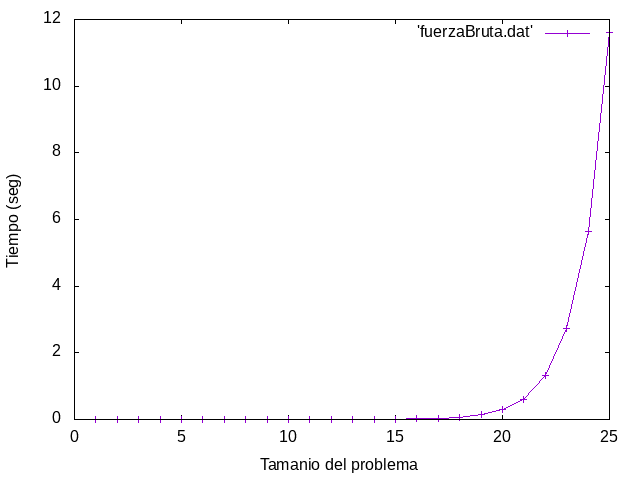
\includegraphics[scale=0.5]{fuerzaBruta.png}
\end{figure}
\end{frame}

\begin{frame}[fragile]{Backtracking sin información}
\begin{figure}[H]
\centering
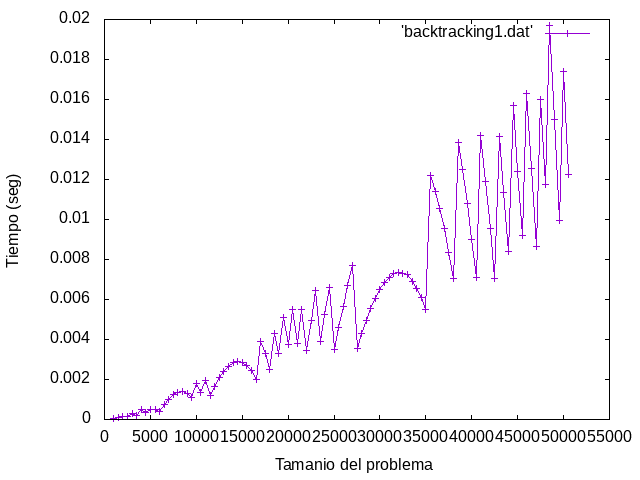
\includegraphics[scale=0.5]{backtracking1.png}
\end{figure}
\end{frame}

\begin{frame}[fragile]{Backtracking con información}
\begin{figure}[H]
\centering
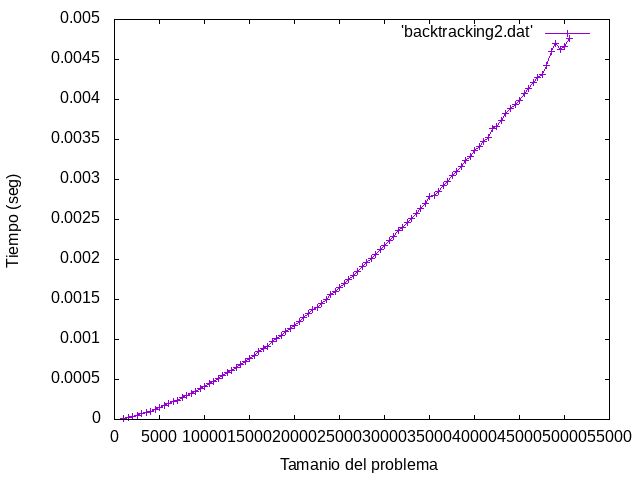
\includegraphics[scale=0.5]{backtracking2.png}
\end{figure}
\end{frame}

\begin{frame}[fragile]{Comparativa de algoritmos}
\begin{figure}[H]
\centering
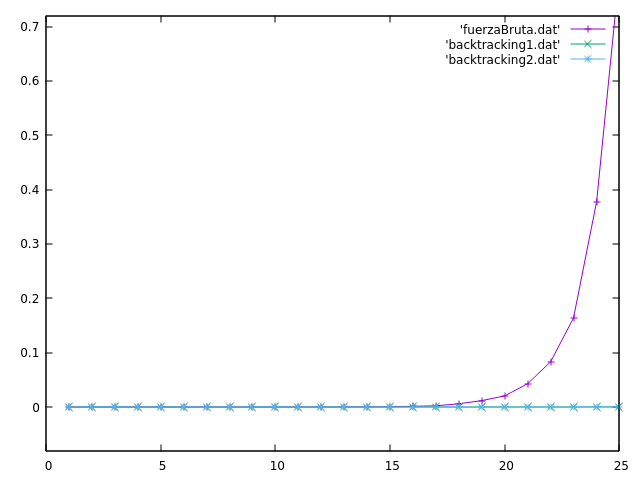
\includegraphics[scale=0.5]{todos.png}
\end{figure}
\end{frame}

\begin{frame}[fragile]{Comparativa de algoritmos backtracking}
\begin{figure}[H]
\centering
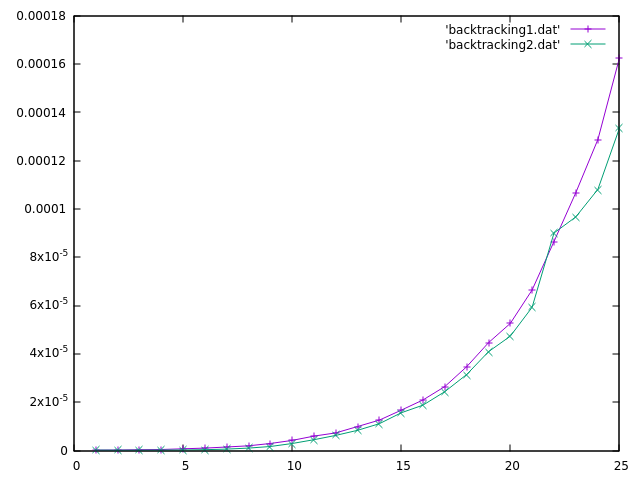
\includegraphics[scale=0.5]{ambos_backtracking.png}
\end{figure}
\end{frame}

\begin{frame}[fragile]{Tiempos obtenidos}
\begin{tabular}{|c|c|}
\hline
\textbf{Algoritmo} & \textbf{Tiempo (s)} \\
\hline
Fuerza bruta & 0,00115\\
\hline
Backtracking sin información & 7,4455$ \cdot 10^{-6}$ \\
\hline
Backtracking con información & 8,9749$ \cdot 10^{-6}$\\
\hline
\end{tabular}
\end{frame}


\section*{Fin de la presentación}

\begin{frame}{Fin}
\begin{center}
\huge{Fin de la presentación}
\end{center}
\end{frame}


\end{document}


